% ============================================================
% NACA AIRFOIL THEORY 
% ============================================================
\section*{NACA Airfoil Theory}

As early as the 1920s, 
research institutions in Europe and the United States began systematic measurements of the aerodynamic characteristics of airfoils in practical use. 
The results were organized into families of airfoils exhibiting specific aerodynamic properties. 
With a catalog of experimentally validated airfoils, 
aircraft designers were able to select suitable profiles efficiently for particular flight applications.

The National Advisory Committee for Aeronautics (NACA) conducted one of the most comprehensive and systematic investigations into the influence of airfoil geometry on aerodynamic performance. 
Early cambered airfoils, 
such as the Clark-Y and Göttingen sections, 
were known from initial wind tunnel experiments to exhibit favorable aerodynamic characteristics. 
NACA adopted these existing profiles as references; 
by removing the camber and normalizing the thickness-to-chord ratio, the resulting geometries became systematically comparable. 
A polynomial curve fit was then used to define the thickness distribution, forming the foundation of many subsequent NACA airfoil families, including the classic NACA 00-series symmetric airfoils.

The airfoil geometry is defined in a Cartesian coordinate system in which the $x$-coordinate is measured along the chord line and normalized by the chord length $c$. 
The leading edge corresponds to $x = 0$, while the trailing edge corresponds to $x = 1$.

The airfoil surfaces are generated by superimposing the thickness distribution $y_t(x)$ onto the mean camber line $y_c(x)$. 
The upper and lower surface coordinates are therefore defined as
\begin{equation}
\begin{aligned}
x_u &= x - y_t \sin \theta, \\
y_u &= y_c + y_t \cos \theta,
\end{aligned}
\label{upper_camber}
\end{equation}

\begin{equation}
\begin{aligned}
x_l &= x + y_t \sin \theta, \\
y_l &= y_c - y_t \cos \theta,
\end{aligned}
\label{lower_camber}
\end{equation}

where the local inclination angle $\theta$ of the mean camber line is given by
\begin{equation}
\theta = \tan^{-1}\left(\frac{dy_c}{dx}\right).
\end{equation}

% ----------------------------------------------------------
% Classical Thickness Distributions
% ----------------------------------------------------------

\subsection*{Classical Thickness Distributions}

% ----- Matching Empirical Curves by Simultaneous Power Equations -----

\subsubsection*{Matching Empirical Curves by Simultaneous Power Equations}

Many important developments in aerodynamics have historically been empirical in nature. 
As theoretical frameworks advanced, 
it became necessary to express these empirical observations in analytical form. 
Notable examples include the thickness equation of the classical NACA four-digit symmetric airfoils, thin-airfoil theory formulations, and spanwise loading distributions. 

In addressing such problems, 
mathematicians rely primarily on two powerful analytical tools: power series expansions and Fourier series representations. 
These methods allow experimentally observed geometric or aerodynamic trends to be approximated using continuous mathematical expressions, 
as mentioned by Alan Pope in \textit{Basic Wing and Airfoil Theory} \cite{basic_wing_and_airfoil_theory}.

\begin{figure}[h]
\centering
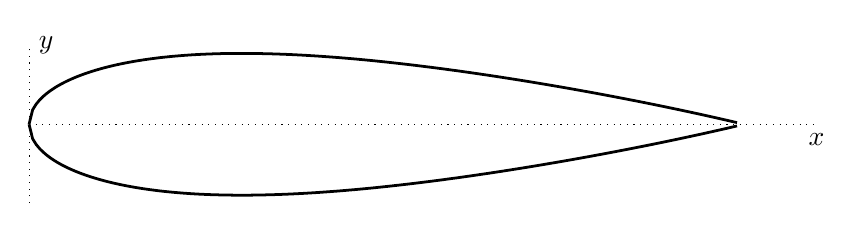
\begin{tikzpicture}[samples=200, domain=0:1]
    % Axes
    \draw[dotted] (0,0) -- (10,0) node[below] {$x$}; 
    \draw[dotted] (0,-1) -- (0,1) node[right] {$y$};
    
    % Thickness distribution (scaled)
    \draw[line width=1pt] 
        plot (9*\x,{9*(0.2969*sqrt(\x) 
        -0.1260*\x 
        -0.3516*\x^2 
        +0.2843*\x^3 
        -0.1015*\x^4)});
        
    \draw[line width=1pt] 
        plot (9*\x,{-9*(0.2969*sqrt(\x) 
        -0.1260*\x 
        -0.3516*\x^2 
        +0.2843*\x^3 
        -0.1015*\x^4)});
\end{tikzpicture}
\caption{NACA 0020 profile}
\end{figure}
To illustrate this procedure, 
consider the development of the NACA 0020 airfoil equation. 
During the period from 1925 to 1935, 
two airfoils with markedly different camber characteristics were widely used: the Göttingen 398 and the Clark Y.
When the camber was removed from these profiles, 
their thickness distributions were found to be nearly identical. 
This observation motivated the adoption of a common thickness distribution combined with various parabolic camber lines 
in order to systematically investigate the influence of maximum camber magnitude and its chordwise location.

A critical step in this process was the formulation of a mathematical expression 
for the basic symmetric thickness shape. The empirical geometric data corresponded 
to a 20 percent thick airfoil defined in a Cartesian coordinate system, with the leading 
edge located at the origin and the trailing edge at $x = 1$.

The empirical conditions were:
\begin{enumerate}
\renewcommand{\labelenumi}{(\arabic{enumi})}
\item Maximum ordinate\\[10pt]
$
x = 0.3, \qquad  y = 1.0, \qquad \displaystyle \frac{dy}{dx} = 0
$

\item Ordinate at the trailing edge\\[10pt]
$
x = 1.0, \qquad y = 0.002
$

\item Trailing edge angle\\[10pt]
$
x = 1.0, \qquad \displaystyle \frac{dy}{dx} = -0.234 
$

\item Nose shape\\[10pt]
$
x = 0.1, \qquad  y = 0.078 
$
\end{enumerate}
Inspection of the nose region suggests that the leading-edge shape may be 
approximated by a square-root function of the form $y = a_0 \sqrt{x}$. 
However, to ensure closure at the trailing edge, a linear correction term 
may be introduced as a first approximation. 
This leads to the preliminary form
\[
y = a_0 \sqrt{x} + a_1 x .
\]

To satisfy all five empirical conditions, higher-order polynomial terms are added, 
yielding the general expression
\[
y = a_0 \sqrt{x}
    + a_1 x
    + a_2 x^2
    + a_3 x^3
    + a_4 x^4 .
\]

Differentiation gives
\[
\frac{dy}{dx}
=
\frac{1}{2} a_0 x^{-1/2}
+ a_1
+ 2 a_2 x
+ 3 a_3 x^2
+ 4 a_4 x^3 .
\]

With five empirical constraints and five unknown coefficients, the resulting 
system of simultaneous equations can be solved to obtain
\[
y =
0.2969 \sqrt{x}
- 0.1260 x
- 0.3516 x^2
+ 0.2843 x^3
- 0.1015 x^4 .
\]

For airfoils of other thickness ratios within the same family, the ordinates of 
the 0.20 thickness-ratio model are scaled by the factor $(t/0.20)$, where $t$ is the ratio of the maximum thickness to the chord, $c$.
\[
\pm\, y_{t} =
\left(\frac{t}{0.2}\right)
\left(
0.2969 \sqrt{x}
- 0.1260 x
- 0.3516 x^2
+ 0.2843 x^3
- 0.1015 x^4 
\right)
\]

The leading-edge radius of this airfoil family is defined as the radius of 
curvature of the basic thickness equation evaluated at $x = 0$. 
Owing to the presence of the term $a_0 \sqrt{x}$, the radius of curvature 
remains finite at the leading edge and can be shown to be
\begin{equation}
R_{LE} = \frac{a_0^2}{2}
\left(\frac{t}{0.2}\right)^2
\equiv 1.1019\, t^2 ,
\end{equation}

which is obtained by taking the limit as $x \to 0$ of the standard expression 
for the radius of curvature,
\[
R = 
\frac{
\left[
1+\left(\displaystyle\frac{dy}{dx}\right)^2
\right]^{3/2}
}{
\left|
\displaystyle \frac{d^2y}{dx^2}
\right|
}.
\]

The trailing-edge angle is defined as the angle between the upper and lower 
surfaces at the trailing edge. It may be expressed as
\begin{equation}
\delta_{TE}
=
2 \tan^{-1}
\left[
\frac{t}{0.2}
\left(
\frac{a_0}{2}
+ a_1
+ 2a_2
+ 3a_3
+ 4a_4
\right)
\right]
\equiv
2 \tan^{-1}(1.0625\, t),
\end{equation}

which is obtained by evaluating the slope of the thickness distribution 
at $x = 1$ (or equivalently $x = c$ in dimensional form).

The local surface inclination at the trailing edge is therefore
\[
\varphi =
\left.
\left|
\frac{dy_t}{dx}
\right|
\right|_{x=1}.
\]

Because the upper and lower surfaces are symmetric with respect to the mean 
camber line for a symmetric airfoil, 
the total trailing-edge angle is 
twice this value, i.e., $\delta_{TE} = 2\varphi$.

% ----- Matching Empirical Curves by Simultaneous Fourier Series -----

\subsubsection*{Matching Empirical Curves by Simultaneous Fourier Series}

A second approach for representing empirical aerodynamic curves employs trigonometric series consisting of sine and cosine terms. 
In many cases, this method is more efficient and mathematically convenient than using exponential relations.

Fourier series are particularly useful in aerodynamic theory because they allow complex distributions to be approximated by a finite number of harmonic terms. 
Two classical applications illustrate this approach.
The first application involves representing a camber line that is not symmetric about the mid-chord. 
In this case, 
a sine series is typically employed since sine terms naturally satisfy boundary conditions at the leading and trailing edges while allowing asymmetric curvature.
The second application concerns the representation of lift distribution along a finite wing that is symmetric about the mid-span. 
In this case, 
a cosine series is commonly used, as cosine functions inherently capture symmetric distributions about the central axis.

By using simultaneous Fourier series, 
empirical aerodynamic curves can be matched with high accuracy while preserving essential physical boundary conditions. 
This approach forms an important theoretical foundation in thin airfoil theory and lifting-line theory.

% ----- Reformulation of Thickness Distribution for Sharp Trailing Edge -----

\subsubsection*{Reformulation of Thickness Distribution for Sharp Trailing Edge}

The classical NACA 4-digit thickness distribution is defined using
a polynomial representation with a small but finite trailing edge thickness.
For the original formulation, 
the trailing edge ordinate at $x=1$
is slightly different from zero due to the coefficient of the $x^4$ term
($-0.1015$), resulting in a finite trailing edge.

In the present work, the geometric condition at the trailing edge
is modified to enforce a sharp trailing edge:
\[
x = 1, \qquad y = 0.
\]

To satisfy this boundary condition, the coefficient of the $x^4$ term
is recalculated such that
\[
0.2969
- 0.1260
- 0.3516
+ 0.2843
- a_4 = 0.
\]

Solving for $a_4$ gives:
\[
a_4 = 0.1036.
\]

Thus, the thickness distribution for a symmetric airfoil
with maximum thickness ratio $t= 0.20$ becomes:
\[
y(x) =
0.2969 \sqrt{x}
- 0.1260 x
- 0.3516 x^2
+ 0.2843 x^3
- 0.1036 x^4 .
\]

For airfoils with other thickness ratios within the same family,
the ordinate distribution is scaled linearly with respect to the
maximum thickness ratio:
\[
\pm y_t(x) =
\left(\frac{t}{0.2}\right)
\left(
0.2969 \sqrt{x}
- 0.1260 x
- 0.3516 x^2
+ 0.2843 x^3
- 0.1036 x^4
\right).
\]

This modification ensures a geometrically sharp trailing edge
while preserving the overall thickness distribution characteristics
of the original NACA formulation.

% ----------------------------------------------------------
% NACA 4-Digit Series
% ----------------------------------------------------------

\subsection*{NACA 4-Digit Series}

The NACA 4-digit series represents the first family of airfoils developed through a systematic mathematical approach to correlate geometry with aerodynamic performance. 
The designation system defines the airfoil through three primary parameters:
the first digit specifies the maximum camber as a percentage of the chord;
the second digit indicates the chordwise location of this maximum camber in tenths of the chord from the leading edge; 
and the final two digits represent the maximum thickness as a percentage of the chord, as described in NACA Report No.~460 \cite{NACA_TR_460}. 

Thus, the NACA 2412—a quintessential wing section for general aviation—
features a maximum camber of 2 percent of the chord located at $0.4$ of the chord from the leading edge, with a maximum thickness of 12 percent of the chord. 
Symmetric airfoils constitute a critical subset of this family where the mean camber line coincides exactly with the chord line. 
Because the maximum camber is zero, the first two digits are denoted as ``00,'' rendering the camber position irrelevant. 
The NACA 0012 is the industry standard for symmetric sections, 
widely utilized for horizontal and vertical stabilizers due to its zero pitching moment at a zero angle of attack and its predictable aerodynamic behavior. 
For simulations requiring a thinner profile to model high-speed tail surfaces, the NACA 0009 serves as a primary representative.

% ----- Mean Camber Line Formulation -----

\subsubsection*{Mean Camber Line Formulation}

The mean camber line of the four-digit series is defined by two parabolic 
segments of the general form
\[
y = b_0 + b_1 x + b_2 x^2 .
\]

The constants are determined from the following boundary conditions:

\bigskip

\textit{(1) Camber-line endpoints}
\begin{align*}
x &= 0, & y &= 0 \\
x &= 1, & y &= 0
\end{align*}

\textit{(2) Maximum camber condition}
\begin{align*}
x &= p, & y &= m
\end{align*}

Thus, the mean camber line is given by

\begin{equation}
y_c =
\begin{cases}
\displaystyle 
\frac{m}{p^2}(2px - x^2),
& 0 \le x \le p \\[12pt]

\displaystyle 
\frac{m}{(1-p)^2}
\left[(1-2p) + 2px - x^2 \right],
& p \le x \le 1
\end{cases}
\label{naca_4-digit_mean_camber}
\end{equation}

The slope of the camber line is obtained by differentiation:

\begin{equation}
\frac{dy_c}{dx} =
\begin{cases}
\displaystyle 
\frac{2m}{p^2}(p - x),
& 0 \le x \le p \\[12pt]

\displaystyle 
\frac{2m}{(1-p)^2}(p - x),
& p \le x \le 1
\end{cases}
\end{equation}

In practical applications, the parameters $m$, $p$, and $t$ may be varied 
to tailor the aerodynamic characteristics of the airfoil. 
Increasing the maximum camber generally enhances the lift coefficient, 
while the camber location influences the pitching moment and pressure distribution. 
The thickness ratio affects structural strength, drag characteristics, and 
leading-edge radius.

By systematically varying these parameters, 
a wide range of airfoils can be generated within the four-digit series 
to meet specific design requirements.

% ----------------------------------------------------------
% NACA 5-Digit Series
% ----------------------------------------------------------

\subsection*{NACA 5-Digit Series}

Following the success of the four-digit family, 
the NACA 5-digit series was developed to push the boundaries of maximum lift capability and aerodynamic efficiency. 
While the series retains the thickness distribution of its predecessor, 
it introduces a significantly more complex mean camber line. 
The primary design objective was to shift the maximum camber substantially forward, 
as experimental data indicated that forward camber placement could drastically increase the maximum lift coefficient ($C_{l_{max}}$) while simultaneously reducing the pitching moment ($C_m$) and minimum profile drag. 
The geometry and aerodynamic characteristics of the five-digit family are studied in NACA Report No.~537 \cite{NACA_TR_537}.

The five-digit designation system reflects these performance-oriented goals. 
The first digit represents the design lift coefficient ($C_{l_i}$) in tenths, multiplied by $3/2$. 
The second and third digits together define the position of the maximum camber, and the final two digits indicate the maximum thickness ratio. 
For simulations, 
the 230-series is the quintessential representative of a "high-lift, low-moment" section.

A specialized sub-family within this series incorporates reflexed camber lines, where the trailing edge curves slightly upward. 
These sections were mathematically derived to produce a near-zero pitching moment about the quarter-chord, 
making them theoretically ideal for tailless or flying-wing configurations where longitudinal stability is a primary concern. 
The NACA 23112 serves as a primary representative of this reflexed geometry. While providing unique stability benefits, 
these sections have seen more limited practical application compared to the standard 230-series due to a slight reduction in maximum lift potential.

% ----- Three-Digit Mean Camber Line -----

\subsubsection*{Three-Digit Mean Camber Line}


To obtain a camber line with a strongly forward maximum camber location, 
the so-called three-digit camber formulation was introduced in NACA Report No.~537 \cite{NACA_TR_537}. 

The camber line is defined in two regions such that the curvature 
(second derivative) decreases linearly to zero at a specified junction 
point $x = m$ and remains zero from that point to the trailing edge.

Thus,

For $0 \le x \le m$:\quad
$
\displaystyle \frac{d^2 y}{dx^2} = k_1 (x - m)
$

For $m \le x \le 1$:\quad
$
\displaystyle \frac{d^2 y}{dx^2} = 0
$

The design constraints are:

\textit{(1) Camber-line endpoints}
\begin{align*}
x &= 0, & y &= 0 \\
x &= 1, & y &= 0
\end{align*}

\textit{(2) Continuity at the junction point $x = m$}
\begin{align*}
y_N &= y_T \\[6pt]
\left( \frac{dy}{dx} \right)_N &= 
\left( \frac{dy}{dx} \right)_T
\end{align*}


where the subscripts $_N$ and $_T$ refer to the fore and aft equations, respectively. 

The resulting camber line is

\begin{equation}
y_c =
\begin{cases}
\displaystyle 
\frac{k_1}{6}
\left[
x^3 - 3mx^2 + m^2(3-m)x
\right],
& 0 \le x \le m \\[12pt]

\displaystyle 
\frac{k_1 m^3}{6}(1-x),
& m \le x \le 1
\end{cases}
\end{equation}

and the slope of the simple camber is

\begin{equation}
\frac{dy_c}{dx} =
\begin{cases}
\displaystyle 
\frac{k_1}{6}
\left[
3x^2 - 6mx + m^2(3-m)
\right],
& 0 \le x \le m \\[12pt]

\displaystyle 
-\frac{k_1 m^3}{6},
& m \le x \le 1.
\end{cases}
\end{equation}

The parameter $m$ is determined such that the maximum camber occurs at chordwise positions $p$ calculated by multiplying the second digit by $0.05$. 
Consequently, 
digits 1 through 5 correspond to standard maximum camber locations at $0.05c$, $0.10c$, $0.15c$, $0.20c$, and $0.25c$, respectively.

The location of maximum camber is obtained from the condition
\[
\left.
\frac{dy_c}{dx}
\right|_{x = p} = 0,
\]
which yields
\[
p
=
m
\left[
1 - \sqrt{\frac{m}{3}}
\right].
\]
The constant $k_1$ is selected to ensure the design lift coefficient ($C_{l_i}$) equals the product of the first digit and $0.15$. 
Accordingly, 
first digits of 1, 2, and 3 correspond to ideal lift coefficients of 0.15, 0.30, and 0.45, respectively.

The tabulated parameters are as follows.
\begin{table}[h!]
\centering

\label{tab:naca5_nonreflex}
\begin{tabular}{|c|c|c|r|}
\hline
Camber-line designation & $p$ & $m$ & \multicolumn{1}{c|}{$k_1$} \\
\hline
210 & 0.05 & 0.0580 & 361.400 \\
220 & 0.10 & 0.1260 & 51.640 \\
230 & 0.15 & 0.2025 & 15.957 \\
240 & 0.20 & 0.2900 & 6.643 \\
250 & 0.25 & 0.3910 & 3.230 \\
\hline
\end{tabular}
\caption{Tabulated parameters of non-reflexed camber lines 
for $C_{l_i}=0.3$}
\end{table}

% ----- Reflexed Mean Camber Line -----

\subsubsection*{Reflexed Mean Camber Line}

To obtain a zero pitching moment about the quarter-chord, 
a reflexed mean line was introduced. 
In this formulation, the curvature is again defined piecewise:

For $0 \le x \le m$:\quad
$
\displaystyle \frac{d^2 y}{dx^2} = k_1 (x - m)
$

For $m \le x \le 1$:\quad
$
\displaystyle \frac{d^2 y}{dx^2} = k_2 (x - m)
$

Solving the related equations yields

\begin{equation}
y_c =
    \begin{cases}
        \displaystyle \frac{k_1}{6}\left[(x - r)^3 - \frac{k_2}{k_1}(1-r)^3x - r^3x + r^3\right], & 0\leq x\leq r \\[15pt]
        \displaystyle \frac{k_1}{6}\left[\frac{k_2}{k_1}\left(x - r\right)^3 - \frac{k_2}{k_1}(1-r)^3x - r^3c + r^3\right],& r\leq x \leq 1 
    \end{cases}
\end{equation}

The slope is derived using differentiation 

\begin{equation}
\frac{dy_c}{dx} =
    \begin{cases}
        \displaystyle \frac{k_1}{6}\left[3(x - r)^2 - \frac{k_2}{k_1}(1-r)^3 - r^3\right], & 0\leq  x\leq r \\[15pt]
        \displaystyle \frac{k_1}{6}\left[3\frac{k_2}{k_1}\left(x - r\right)^2 - \frac{k_2}{k_1}(1-r)^3 - r^3\right], & r\leq \displaystyle x \leq 1 
    \end{cases}
\end{equation}

Imposing the condition of a zero slope at the maximum camber location,
\[
\left.
\frac{dy_c}{dx}
\right|_{x = p}
= 0,
\]
leads to
\[
\frac{k_2}{k_1}
=
\frac{
3(m-p)^2 - m^3
}{
(1-m)^3
}.
\]

For each prescribed value of $p$, the parameter $m$ was determined 
to satisfy the condition of zero quarter-chord pitching moment 
($C_{m_{c/4}} = 0$). 
Subsequently, 
$k_1$ was evaluated to produce a design lift coefficient of $C_{l_i} = 0.3$.

The tabulated values of $m$, $k_1$, and $k_2/k_1$ 
are summarized above.

\begin{table}[h!]
\centering
    \begin{tabular}{|c|c|c|r|l|}
        \hline
        Camber-line designation & $p$ & $m$ & \multicolumn{1}{c|}{$k_1$} & \multicolumn{1}{c|}{$k_2/k_1$}  \\
        \hline
        211 & 0.05 & - & \multicolumn{1}{c|}{-} & \multicolumn{1}{c|}{-} \\
        221 & 0.10 & 0.1300 & 51.990 & 0.000764 \\
        231 & 0.15 & 0.2170 & 15.793 & 0.00677 \\
        241 & 0.20 & 0.3180 & 6.520 & 0.0303 \\
        251 & 0.25 & 0.4410 & 3.191 & 0.1355 \\
        \hline
    \end{tabular}
    \caption{Tabulated coefficients of reflexed camber for $C_{l_i}=0.3$}
\end{table}

In practical design applications, the defining parameters of the 
five-digit series are not restricted to the tabulated integer values. 
Instead, 
they may be treated as continuous variables to achieve 
specific aerodynamic requirements. 
By adjusting the camber magnitude, camber location, and thickness 
ratio, designers can tailor the lift characteristics, pitching 
moment behavior, and drag performance to meet particular mission 
profiles.
Thus, 
although originally defined by discrete designations, 
the five-digit formulation provides a flexible analytical framework 
for systematic airfoil development.

% ----------------------------------------------------------
% NACA 4- and 5-Digit Modified Series
% ----------------------------------------------------------

\subsection*{NACA 4- and 5-Digit Modified Series}

The modified NACA four- and five-digit airfoil families were developed 
to provide greater geometric flexibility 
while preserving the basic thickness characteristics of the original series. 

In the modified designation, 
the airfoil number is followed by a dash and a two-digit suffix (e.g., NACA 0012-63). 
The first digit after the dash represents the leading edge radius index, and the second digit 
indicates the location of maximum thickness in tenths of the chord 
measured from the leading edge, which is represented in NACA Report No.~492 \cite{NACA_TR_492}.

As in the original four-digit series, the ordinates vary linearly 
with the thickness–chord ratio. 
Thus, for any desired thickness ratio $t/c$, the ordinates 
are obtained by scaling the design thickness distribution 
proportionally.
The original NACA four-digit series is a special case of the modified 
formulation corresponding to: leading edge index $I = 6$ (normal leading edge) and maximum thickness location at $0.30c$.
Hence, the classical four-digit airfoil can be interpreted as 
a particular instance of the more general modified family.

% ----- Thickness Distributions -----

\subsubsection*{Thickness Distributions}

The thickness distribution is defined piecewise so that the leading-edge 
radius and the chordwise location of maximum thickness may be varied 
independently.

Similar to the thickness distributions formulation of NACA 4-digit and 5-digit series, a critical step in this process was the formulation of a mathematical expression 
for the basic symmetric thickness shape. The empirical geometric data corresponded 
to a 20\% thick airfoil defined in a Cartesian coordinate system.

If the chord is taken at the position $x$ axis from $0$ to $1$, the ordinates y from the leading edge to the maximum thickness location 
($0 \le x \le m$):
\[
\pm\, y_t =
a_0 \sqrt{x}
+ a_1 x
+ a_2 x^2
+ a_3 x^3,
\]

From the maximum thickness location to the trailing edge 
($m \le x \le 1$):
\[
\pm\, y_t =
d_0
+ d_1 (1-x)
+ d_2 (1-x)^2
+ d_3 (1-x)^3.
\]

The constants are determined from the following geometric constraints:

\begin{enumerate}
\renewcommand{\labelenumi}{(\arabic{enumi})}
\item Specified maximum thickness\\[10pt]
$ 
x=m \qquad y=0.10 \qquad \displaystyle \frac{dy}{dx}=0
$

\item Prescribed leading-edge radius\\[10pt]
$
x=0 \qquad \displaystyle R=\frac{a_0^2}{2}
$
\item Specified radius of curvature at the point of maximum thickness\\[10pt]
$
x=m \qquad \displaystyle R=\frac{(1-m)^2}{2d_1(1-m)-0.588}
$
\item Specified trailing-edge ordinate\\[10pt]
$
x=1 \qquad y=d_0=0.002
$
\item Prescribed trailing-edge angle\\[10pt]
$
x=1 \qquad \displaystyle \frac{dy}{dx}=d_1=f(m)
$
\end{enumerate}

These conditions ensure continuity of ordinate, slope, and curvature 
at the junction point $x = m$.

\begin{table}[h!]
\centering
\label{tab:d1_values}
\begin{tabular}{|c|c|}
\hline
$m$ & $d_1$ \\
\hline
0.2 & 0.200 \\
0.3 & 0.234 \\
0.4 & 0.315 \\
0.5 & 0.465 \\
0.6 & 0.700 \\
\hline
\end{tabular}
\caption{Selected values of $d_1$ to prevent curvature reversal \cite{NACA_TR_492}}
\end{table}

Some approximations of the coefficients above were described by William H.Mason in his book \textit{Lecture Notes on Configuration Aerodynamics} \cite{configuration_aerodynamics} as follows.

The Riegels approximate $d_1$ is define by
\[
d_1=f(m) \cong \frac{(2.24-5.42m+12.3m^2)}{10(1-0.878m)}
\]

Once the value of $d_1$ is known, $d_2$ and $d_3$ are found from the relations given by Riegels:
\[
d_2=\frac{0.294-2(1-m)d_1}{(1-m)^2}
\]

and 
\[
d_3=\frac{-0.196+(1-m)d_1}{(1-m)^3}
\]

With the $d_i$ coefficients determined, the $a_i$ coefficients can be found. First, $a_0$ is based on the leading edge radius:
\[
\begin{aligned}
a_0 &=0.2969 \, \frac{I}{6}, & \text{for }I\leq8\\
& =0.2969\sqrt{3} ,  & \text{for }I=9
\end{aligned}
\]

Define the following
\[
\rho_1=\frac{1}{5}\frac{(1-m)^2}{[0.588-2d_1(1-m)]}
\]

then the remaining coefficients can be found from:
\[
a_1=
\frac{0.3}{m}
-\frac{15}{8}\cdot\frac{a_0}{m}
-\frac{m}{10\rho_1}
\]

\[
a_2=
-\frac{0.3}{m^2}
+\frac{5}{4}\cdot\frac{a_0}{m^{3/2}}
+\frac{1}{5\rho_1}
\]

\[
a_3=
\frac{0.1}{m^3}
-\frac{0.375a_0}{m^{5/2}}
-\frac{1}{10\rho_1m}
\]

% ----- Reformulated Thickness Distribution (Sharp Trailing Edge) -----

\subsubsection*{Reformulated Thickness Distribution (Sharp Trailing Edge)}

For the classical finite trailing-edge formulation,
\[
x=1 \qquad y=d_0=0.002 .
\]

To enforce a geometrically sharp trailing edge, the boundary condition is modified to
\[
x=1 \qquad y=d_0=0 .
\]

The coefficients $d_2$ and $d_3$ are obtained from the geometric constraints
at $x=m$ and $x=1$.
For the general case,
\[
d_2=\frac{3(0.1-d_0)-2(1-m)d_1}{(1-m)^2}
\]

\[
d_3=\frac{2(d_0-0.1)+(1-m)d_1}{(1-m)^3}
\]

Substituting $d_0=0$ for the sharp trailing edge gives
\[
d_2=\frac{0.3-2(1-m)d_1}{(1-m)^2}
\]

\[
d_3=\frac{-0.2+(1-m)d_1}{(1-m)^3}
\]

This modification affects only the aft thickness distribution.
Since the leading-edge geometry and the maximum thickness conditions
remain unchanged, the coefficients $a_i$ derived previously are preserved.

% --- Leading-Edge Radius and Trailing-Edge Angle

\subsubsection*{Leading-Edge Radius and Trailing-Edge Angle}

The leading-edge index $I$ controls the magnitude of the leading-edge 
radius and is proportional to the coefficient $a_0$.

The relationship between the leading-edge radius $R_{LE}$ and 
the index number $I$ is given by
\[
R_{LE}
=
\frac{1}{2}
\left(
0.2969\,
\frac{t}{0.2}\,
\frac{I}{6}
\right)^2.
\]

\begin{table}[h!]
\centering
\label{tab:le_index}
\begin{tabular}{|l|c|l|}
\hline
\multicolumn{1}{c|}{Type} & Leading-edge Index $I$ & \multicolumn{1}{c|}{$a_0$}\\
\hline
Sharp & 0 & 0 \\
Quarter-normal & 3 & 0.148450 \\
Normal & 6 & 0.296900 \\
Three-times normal & 9 & 0.514246 \\
\hline
\end{tabular}
\caption{Leading-edge index classification}
\end{table}

The trailing-edge angle depends on the position of maximum thickness, $m$, and is given by
\[
\delta_{TE} =2\tan^{-1}{(d_1)} = 2\tan^{-1}{[f(m)]}
\]

% ----- Modified Five-Digit Series -----

\subsubsection*{Modified Five-Digit Series}

The modified five-digit airfoils retain the same camber-line 
definitions as the standard five-digit series but incorporate 
the modified thickness formulation described above.

Thus, 
the camber line is defined according to the five-digit 
design equations, while the thickness distribution is replaced 
by the modified polynomial expressions that allow independent 
control of: leading-edge radius, maximum thickness location, and trailing-edge angle. 
This combination provides increased flexibility in tailoring airfoil geometry for specific aerodynamic performance requirements.

In practical aerodynamic design, the modified formulation allows 
the defining parameters to be treated as continuous variables 
rather than discrete tabulated values.
By adjusting the camber magnitude, camber location, thickness ratio, 
leading-edge radius, and maximum thickness position, designers 
can systematically optimize lift characteristics, drag performance, 
and pitching moment behavior.
Consequently, the modified NACA families provide a versatile 
analytical framework for preliminary airfoil design.

% ----------------------------------------------------------
% NACA 1-Series Airfoils and 16-Series Designation
% ----------------------------------------------------------

\subsection*{NACA 1-Series Airfoils and 16-Series Designation}

Unlike previous airfoil families defined by geometric polynomials, the NACA 1-Series was developed using inverse design methods rooted in advanced aerodynamic theory. 
By the late 1930s, research shifted from prescribing geometry to specifying a desired pressure distribution and mathematically deriving the corresponding shape. This approach allowed designers to tailor the airfoil to specific performance targets, such as lift-to-drag ratios and stall behavior, rather than relying on empirical geometric iterations. 
Consequently, 1-Series airfoils are generated numerically rather than through simple analytical expressions, as documented in NACA Report No.~824 \cite{NACA_TR_824}.

The identification of the 1-Series follows a five-digit convention, exemplified by the NACA 16-212. 
The initial digit "1" denotes the series, while the second digit indicates the chordwise location of minimum pressure in tenths of the chord; in this instance, "6" signifies that minimum pressure occurs at $0.6c$. Following the hyphen, the third digit represents the design lift coefficient in tenths ($C_{L,design}=0.2$), and the final two digits indicate the maximum thickness ratio ($t/c=0.12$).

The 16-Series constitutes the most practically significant subset of this family, optimized to maintain favorable pressure gradients over an extended portion of the chord. 
By shifting the minimum pressure point further aft, these airfoils reduce the suction peak at the leading edge, thereby delaying drag divergence and boundary layer separation at high subsonic speeds. 
While the thickness distribution of the 16-Series shares similarities with the modified 4-digit series, specifically regarding leading-edge radii and mid-chord maximum thickness, its camber line is strictly dictated by aerodynamic requirements \cite{NACA_TR_492}. 
Due to their widespread adoption in high-speed applications, the 16-Series is often categorized independently in contemporary aeronautical literature.

% ----------------------------------------------------------
% NACA 6-Series and 6A-Series
% ----------------------------------------------------------

\subsection*{NACA 6-Series and 6A-Series}

While earlier NACA iterations utilized approximate theoretical methods, they often failed to precisely achieve the pressure distributions required for significant drag reduction. 
The development of the NACA 6-Series represented a transition toward rigorous inverse airfoil theory. 
By prescribing an ideal pressure distribution first and then deriving the corresponding geometry, engineers sought to maximize the extent of the laminar boundary layer. 
This design philosophy focuses on maintaining a favorable pressure gradient over a substantial portion of the chord, thereby minimizing skin-friction drag and producing the characteristic "low-drag bucket", a discrete range of lift coefficients ($C_l$) where the airfoil operates with exceptional efficiency.

The 6-Series designation reflects this complexity, as seen in the example NACA 64$_1$-212, $a=0.6$. The first digit ``6'' identifies the series, while the second digit (``4'') locates the minimum pressure at $0.4c$. 
The subscript (``1'') indicates the width of the low-drag bucket, specifically maintaining laminar flow over a range of $\pm 0.1$ about the design lift coefficient. 
Following the hyphen, the digit ``2'' specifies a design lift coefficient ($C_{l_i}$) of $0.2$, and the final two digits (``12'') denote a thickness ratio ($t/c$) of $0.12$. 
The parameter $a$ defines the fraction of the chord over which the pressure gradient remains favorable; for $a=0.6$, this gradient is maintained over 60 percent of the chord \cite{NACA_TR_824}.

% ----- NACA 6A-Series -----

\subsubsection{NACA 6A-Series}

The 6A-Series was subsequently developed to address the manufacturing and structural limitations of the original 6-Series. 
In the standard 6-Series, the theoretical derivation often resulted in a thin, concave "cusp" near the trailing edge, which was difficult to fabricate and prone to structural failure. 
The 6A-series modifies this by eliminating the trailing edge cusp, resulting in a geometry that is nearly straight from approximately 80 percent chord to the trailing edge. 
This modification simplifies production and improves the pitching moment characteristics while preserving most of the laminar flow benefits.

% ----- Camber Line -----

\subsubsection*{Camber Line}

Unlike the four-digit and five-digit airfoil families, the camber line of the NACA 6-Series airfoils is not defined using simple polynomial expressions. 
Instead, the camber line is determined using inverse aerodynamic design methods to achieve the specified pressure distribution corresponding to the desired design lift coefficient. 
The camber distribution is calculated numerically using thin airfoil theory and potential flow analysis.

The mean lines commonly used with the NACA 6-series airfoils produce a uniform chordwise loading from the leading edge to the point $x=a$ and a linearly decreasing load from this point to the trailing edge. 
Data for NACA mean lines with values of a equal to 0, 0.1, 0.2, 0.3, 0.4, 0.5, 0.6, 0.7, 0.8, 0.9, and 1.0 are presented in the
supplementary figures. 
The ordinates were computed using the following formula, which represents a simplification of the original expression for mean-line ordinates given NACA Report No.~824 \cite{NACA_TR_824}:

\begin{equation*}
\begin{aligned}
y &= 
\frac{C_{l_i}}{2\pi (1+a)}
\Bigg\{
\frac{1}{1-a}
\Bigg[
\frac{1}{2}(a-x)^2 \ln(a-x)  \\
&\quad
-\frac{1}{2}(1-x)^2 \ln(1-x)
+\frac{1}{4}(1-x)^2  
-\frac{1}{4}(a-x)^2
\Bigg] \\
&\quad
- x \ln x
+ g - hx
\Bigg\}
\end{aligned}
\end{equation*}

where 
\[
\begin{aligned}
g &= 
-\frac{1}{1-a}
\left[
a^2
\left(
\frac{1}{2}\ln{a}
+\frac{1}{4}
\right)
+\frac{1}{4}
\right] \\[8pt]
h &= 
\frac{1}{1-a}
\left[
\frac{1}{2}(1-a)^2\ln{(1-a)}
-\frac{1}{4}(1-a)^2
\right]
+g
\end{aligned}
\]

and
\[
\frac{dy}{dx}=
\frac{C_{l_i}}{2\pi(1+a)}
\left\{
\frac{1}{1-a}
\left[
(1-x)\ln{(1-x)}
-(a-x)\ln{(a-x)}
\right]
-\ln{x}
-1
-h
\right\}
\]

The associated angle of attack is 
\[
\alpha_i=
\frac{C_{l_i}h}{2\pi(1+a)}
\]

% ----- Thickness Distributions -----

\subsubsection*{Thickness Distributions}

Similarly, the thickness distribution of the NACA 6-series airfoils was derived using theoretical aerodynamic methods rather than empirical geometric fitting. 
The design procedure was based on potential flow theory and conformal mapping techniques from complex analysis to generate airfoil shapes capable of producing prescribed pressure distributions. 
The derivation methods are introduced in NACA Report No.~824 \cite{NACA_TR_824}, and a detailed theoretical analysis is presented in \textit{Basic Wing and Airfoil Theory} \cite{basic_wing_and_airfoil_theory} and \textit{Theory of Wing Sections} \cite{theory_of_wing_sections}.

The mathematical foundation of this design approach relies on conformal transformation techniques, which enable the mapping of simple analytical flow solutions into airfoil geometries with specific aerodynamic characteristics. 
These transformations preserve the governing equations of inviscid, irrotational flow while reshaping the geometry. 
As a result, they allow designers to control pressure gradients, ensure smooth pressure recovery, and promote extended laminar flow over a significant portion of the airfoil surface.

One of the classical derivation methods in thin airfoil theory is the Joukowski transformation, a conformal mapping used to generate the Joukowski airfoil from a circular cylinder in the complex plane. 
Although the NACA 6-series airfoils are not simple Joukowski profiles, the theoretical framework is conceptually similar. 
Conformal mapping techniques provide the analytical basis for determining thickness distributions that correspond to specified pressure distributions.